\documentclass[11pt,aspectratio=169]{beamer}

\usepackage[T1]{fontenc}
\usepackage{lmodern}
\usepackage{graphicx}
\usepackage{tikz}
\usetikzlibrary{arrows.meta,positioning,calc,decorations.pathreplacing,overlay-beamer-styles,shapes.geometric,patterns}
\usepackage{pgfplots}
\pgfplotsset{compat=1.17}
\usepackage{amsmath,amssymb,mathtools}
\usepackage{booktabs}
\usepackage{array}
\usepackage{multirow}
\usepackage{appendixnumberbeamer}

\setbeamercovered{transparent=5}
\setbeamertemplate{navigation symbols}{}
\setbeamertemplate{itemize items}[circle]
\setbeamertemplate{itemize subitem}{--}
\setbeamertemplate{footline}[frame number]
\setbeamerfont{framesubtitle}{size=\small}
\setbeamercolor{block title}{fg=black,bg=white!80!black}
\setbeamercolor{block body}{fg=black,bg=white!97!black}
\linespread{1.2}
\newcommand{\sym}[1]{\ifmmode^{#1}\else\(^{#1}\)\fi}
\definecolor{citecolor}{RGB}{110,110,165}
\newcommand{\cit}[1]{{\color{citecolor}#1}}

\title{Fertility and Housing Tenure Choice}
\author{Tommaso De Santo}
\date{05/29/2026}

\begin{document}

{
\setbeamertemplate{footline}{}
\maketitle
}

\begin{frame}{Housing and Fertility}
\begin{center}
\includegraphics[width=0.45\textwidth]{../../Latex/newsweek.png}\hspace{-1em}%
\includegraphics[width=0.45\textwidth]{../../Latex/housingwire.png}\\[-0.8em]
\includegraphics[width=0.45\textwidth]{../../Latex/vox.png}\hspace{-1em}%
\includegraphics[width=0.45\textwidth]{../../Latex/cityjournal.png}
\includegraphics[width=0.8\textwidth]{../../Latex/times.png}
\end{center}
\end{frame}

\begin{frame}{Housing, Fertility, and Tenure Choice}
\textbf{Housing costs affect fertility}, but tenure and wealth matter:
\begin{itemize}
  \item Owners have more kids when house prices or housing wealth rise; renters do not \cit{(Dettling \& Kearney 2014)}
  \item Easier mortgage credit raises buying and births jointly, through large-home purchases \cit{(Hacamo 2021, Couillard 2025)}
\end{itemize}
\medskip
Children increase how big of a house you need. This has implications for:
\begin{itemize}
  \item Owning: tenure segmentation
  \item Location: housing cost differs geographically
  \item Wealth: borrowing constraints, bequests
\end{itemize}
\vfill
Physical space is key. How much does it affect fertility?\\
What kind of housing policy is good for natality?\\
\hspace{2em} $\rightarrow\;$ focus on space constraints and tenure choice
\end{frame}

\begin{frame}{This Paper}
Need a structural model where tenure, location, and fertility are joint.
Today:
\vfill
\alert{Model:} lifecycle model of fertility, location, tenure, and saving
\begin{itemize}
  \vfill \item Childbirth creates a jump in housing need
  \vfill \item Housing markets with borrowing constraints, tenure choice, transaction costs
  \vfill \item Location and tenure respond to family-space need
\end{itemize}

\vfill
\alert{Empirics:} document facts about fertility, housing, and moving
\begin{itemize}
  \vfill \item ACS: parents live less in the center; role of center-periphery gaps
  \vfill \item PSID: first birth raises ownership, rooms, and moves for space
\end{itemize}

\vfill
\alert{Goal:} write a model disciplining these interactions, think about policy.
\end{frame}

\section{Model}

\begin{frame}[plain,c,noframenumbering]
\centering
{\Large\textbf{Model}}
\end{frame}

\begin{frame}{Environment}
\begin{itemize}
  \item Two locations: \textbf{center} $(C)$ and \textbf{periphery} $(P)$ within a metro area
  \begin{itemize}
    \item Center has an amenity premium but less elastic housing supply
    \item Common wages; sorting driven by amenities, housing costs, and moving frictions
  \end{itemize}
  \item Adult age $a \in [0,J]$; deterministic aging and death
  \begin{itemize}
    \item Working age $a \in [0, J_R]$; fertile window $a \in [J_f^{\mathrm{start}}, J_f^{\mathrm{end}}]$
    \item Children do not work; they depend on their parents
  \end{itemize}
  \item Households choose:
  \begin{itemize}
    \item \textbf{Fertility}: $n' \in \{0,1,\ldots,\bar n\}$, subject to EV shocks
    \item \textbf{Location}: center or periphery each period (with moving costs and EV shocks)
    \item \textbf{Tenure}: rent or buy a discrete house size $H_k$ on a housing ladder
    \item \textbf{Saving}: liquid wealth $b$ with collateral borrowing for owners
  \end{itemize}
  \item Children age stochastically through life stages; housing need depends on children
\end{itemize}
\end{frame}

\begin{frame}{Preferences}
\small
$n$: fertility; $s$: child-aging stage (stochastic); $m = m(n,s)$: children currently at home.

\medskip
\textbf{Flow utility.} Over consumption and housing services:
\[
u(c,\mathbf h;m)
= \frac{\Big[\big(c-\bar c(m)\big)^\alpha \big(\mathbf h-\bar h(m)\big)^{1-\alpha}\Big]^{1-\sigma}}{1-\sigma}
+ \psi_{\mathrm{child}}\,m.
\]

\textbf{Subsistence requirements.} Depend on family size:
\[
\bar c(m)=\bar c_0+\bar c_1 m,
\qquad
\bar h(m)=\bar h_0+\underbrace{\bar h_{\mathrm{jump}}\mathbf{1}\{m\geq 1\}}_{\text{first-child housing margin}}+\bar h_1 m.
\]

\textbf{Housing services.} Households either rent or own; owners get a service premium:
\[
\mathbf h = \underbrace{\mathbf{1}\{\text{own}\}\,\chi\, h}_{\text{owner services}} + \underbrace{\mathbf{1}\{\text{rent}\}\,h^R}_{\text{renter services}}, \quad \chi > 1.
\]

\begin{itemize}
  \item Child costs disappear after children mature.
\end{itemize}
\end{frame}

\begin{frame}{Bequests}
\small
Terminal utility at death:
\[
\mathcal B(\widetilde b,n)= \theta_0\big(1+\theta_n n\big)\frac{(\theta_1+\widetilde b)^{1-\sigma}}{1-\sigma},
\qquad
\widetilde b=b+(1-\psi)p_i h.
\]
\begin{itemize}
  \vfill \item $\theta_0$ governs overall bequest motive (saving level).
  \vfill \item $\theta_n$ governs the parent--childless saving differential.
  \vfill \item Total bequeathable wealth $\widetilde b$ includes housing equity net of the transaction cost for owners.
\end{itemize}
\end{frame}

\begin{frame}{Housing, Tenure, and Budget Constraints}
\small
\setlength{\abovedisplayskip}{3pt}\setlength{\belowdisplayskip}{3pt}
Households choose housing inputs:
\[
h^R \in \{0, H^R_1,\ldots,H^R_{N_R}\},
\qquad
h \in \{0, H_1,\ldots,H_{N_H}\}.
\]
A household either rents ($h^R>0$, $h=0$) or owns ($h>0$, $h^R=0$).

\smallskip
\textbf{Tenure segmentation:} $\max H_k > \max H^R_j$, so family-sized housing is reachable only through ownership.

\smallskip
\textbf{Renters} ($h=0$)
\[
b' = qb + y(a) - c - r_i h^R,
\qquad b' \geq 0.
\]

\textbf{Owners} ($h^R=0$), with prior owner stock $h_{-1}$
\[
b' = qb + y(a) - c - (\delta+\tau_H)\,p_i h - \mathbf{1}\{h \neq h_{-1}\}\big[p_i h - (1-\psi)\,p_i h_{-1}\big],
\qquad b' \geq -\phi\,p_i h.
\]

\smallskip
\begin{itemize}\setlength\itemsep{2pt}
  \item $q$: gross bond rate; $\delta$: depreciation; $\tau_H$: property tax; $\psi$: transaction cost.
  \item Movers and newly matured children arrive as renters, then re-choose.
\end{itemize}
\end{frame}

\begin{frame}{Fertility and Child Aging}
\begin{itemize}
  \item Fertility choices are made only in the fertile window $a \in [J_f^{\mathrm{start}},J_f^{\mathrm{end}}]$.
  \item One-shot fertility: can have multiple kids, but choose only once:
  \[
  n' \in \{0,1,\ldots,\bar n\}.
  \]
  \item After birth, children age through stages $s$ (think toddler $\to$ child $\to$ teen $\to$ adult):
  \begin{itemize}
    \item Aging is \textbf{sequential}: each stage transitions only to the next one, with random arrival
    \item All $n'$ children of a parent age \textbf{together} as a single cohort --- $s$ is shared.
  \end{itemize}
  \item While children are at home ($s < $ matured), they raise housing need $\bar h(m)$ and consumption cost $\bar c(m)$.
  \item Once matured, child costs shut off and children enter the economy at age $a=0$.
\end{itemize}
\end{frame}

\begin{frame}{Firms and Earnings}
\small
\begin{itemize}
  \item Competitive firms produce with labor:
  \[
  Y = A L, \qquad w = A.
  \]
  \item \textbf{Common wages} across locations: sorting driven entirely by amenities and housing costs.
  \item Age-dependent earnings:
  \[
  y(a) = \begin{cases} (1-\tau_{\mathrm{pay}})\,w(a) & a < J_R \\ \bar b & a \geq J_R \end{cases}
  \]
  \item Retirees receive a stationary pay-as-you-go pension $\bar b$ financed by payroll taxes.
\end{itemize}
\end{frame}


\begin{frame}{Housing Supply and Price Mapping}
\small
Housing supply in each location:
\[
H_i^s(r_i) = \bar r_i r_i^{\eta_i},
\qquad i \in \{C,P\}.
\]
\begin{itemize}
  \item Less elastic center supply makes family space more expensive in the core.
  \item House prices map into user costs through
  \[
  r_i = (q+\delta+\tau_H)p_i.
  \]

\end{itemize}
\end{frame}

\begin{frame}[t]{%
\only<1>{The Household's Problem}%
\only<2>{The Household's Problem: Housing and Saving}%
\only<3>{The Household's Problem: Location Choice}%
\only<4>{The Household's Problem: Fertility Choice}%
}
% ---------- FLOW DIAGRAM ----------
\vspace{0.3em}
\centering
\scalebox{0.85}{%
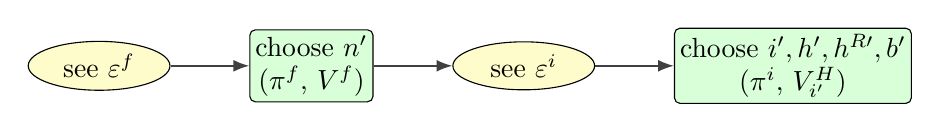
\begin{tikzpicture}[
  node distance=7mm and 10mm, >=Latex,
  see/.style={
    ellipse, draw, fill=yellow!20,
    minimum height=1.3em, minimum width=1.8cm,
    inner sep=2pt, align=center, font=\normalsize
  },
  choose/.style={
    rectangle, draw, fill=green!15, rounded corners=2pt,
    minimum height=1.5em, minimum width=1cm,
    inner sep=2pt, align=center, font=\normalsize
  },
  line/.style={-Latex, semithick, draw=black!75}
]
\node (fertS) [see,    alt=<4>{draw=red, ultra thick}{}] {see $\varepsilon^f$};
\node (fertD) [choose, right=of fertS, alt=<4>{draw=red, ultra thick}{}] {choose $n'$\\($\pi^f$, $V^f$)};
\node (locS)  [see,    right=of fertD, alt=<3>{draw=red, ultra thick}{}] {see $\varepsilon^i$};
\node (locD)  [choose, right=of locS,  alt=<2-3>{draw=red, ultra thick}{}] {choose $i',h',h^{R\prime},b'$\\($\pi^i$, $V^H_{i'}$)};

\draw[line] (fertS) -- (fertD);
\draw[line] (fertD) -- (locS);
\draw[line] (locS)  -- (locD);
\end{tikzpicture}%
}

\vspace{0.35em}
\raggedright
% ---------- EQUATIONS: one per overlay ----------
\setlength{\abovedisplayskip}{4pt}\setlength{\belowdisplayskip}{4pt}

\only<1>{%
\small
\setlength{\abovedisplayskip}{6pt}\setlength{\belowdisplayskip}{6pt}

\textbf{State.}
\[
x=(b,h,i,a,n,s), \qquad h \in \{0,H_1,\dots,H_{N_H}\}.
\]

\begin{itemize}\setlength\itemsep{3pt}
  \item $b$: liquid wealth; $h$: owner-occupied size ($h=0$ if renter); $i$: location; $a$: age.
  \item $n$: fertility; $s$: child-aging stage.
  \item After the fertility choice, $n'$ is the period's fertility state; if no birth, $n'=n$.
\end{itemize}

\medskip
\textbf{Within the period:} choose $n'$, then $(i',h',h^{R\prime},b')$.\\[2pt]
A renter sets $h'=0$; an owner sets $h^{R\prime}=0$.
}

\only<2>{%
{\footnotesize
\setlength{\abovedisplayskip}{6pt}\setlength{\belowdisplayskip}{6pt}

\textbf{Conditional on destination $i'$:}
\[
V^H_{i'}(b,h,i,a,n',s)
=
\max_{h',h^{R\prime},b'}
\;u\big(c,\,\chi h' + h^{R\prime};\,m(n',s)\big)
+ \beta \,\mathbb E_{s'}\!\left[V(b',h',i',a+1,n',s')\right]
\]

\smallskip
\begin{itemize}\setlength\itemsep{3pt}
  \item Owner stock $h' \in \{0,H_1,\dots,H_{N_H}\}$; rental flow $h^{R\prime} \in \{0,H^R_1,\dots,H^R_{N_R}\}$.
  \item Adjustment indicator $\tau = \mathbf{1}\{h'\neq h\;\text{or}\;i'\neq i\}$.
\end{itemize}

\smallskip
\textbf{Budget and collateral.}
\[
\begin{aligned}
c + b' + r_{i'} h^{R\prime} + (\delta+\tau_H)\,p_{i'} h'
&= qb + y(a) - \tau\big[p_{i'} h' - (1-\psi)\,p_i h\big],\\
b' &\geq -\phi\,p_{i'} h'.
\end{aligned}
\]
}
}

\only<3>{%
{\scriptsize
After fertility choice $n'$, draw destination taste shocks
$\varepsilon^i_{i'}$ and choose a destination. Let
\[
\widetilde V_{i'}=V^H_{i'}(b,h,i,a,n',s)+E^R_{i'}-\mu_{ii'}.
\]
The location object is the expected maximum over those shocks:
\[
\begin{aligned}
V^{i}(b,h,i,a,n',s)
&\equiv
\mathbb E_{\varepsilon^i}\max_{i'\in\{C,P\}}
\left\{\widetilde V_{i'}+\varepsilon^i_{i'}\right\}\\
&\propto
\kappa_i\ln\sum_{i'\in\{C,P\}}
\exp\!\left(\frac{\widetilde V_{i'}}{\kappa_i}\right).
\end{aligned}
\]
\vspace{-0.5em}
\begin{itemize}\setlength\itemsep{1pt}
  \item $V^H_{i'}$ maximizes over $(h', h^{R\prime}, b')$ in destination $i'$.
\end{itemize}
\vspace{-0.4em}
Choice probabilities:
\[
\pi_{i'}^{i}(b,h,i,a,n',s)
=
\frac{\exp\!\left(\widetilde V_{i'}/\kappa_i\right)}
{\sum_{j\in\{C,P\}}\exp\!\left(\widetilde V_j/\kappa_i\right)}.
\]
}
}

\only<4>{%
{\footnotesize
\setlength{\abovedisplayskip}{6pt}\setlength{\belowdisplayskip}{6pt}

Childless households in the fertile window choose fertility once:
\[
\begin{aligned}
V(b,h,i,a,0,0)
&\equiv
\mathbb E_{\varepsilon^f}\max_{n'\in\mathcal N}
\left\{V^{i}(b,h,i,a,n',s(n'))+\varepsilon^f_{n'}\right\}\\[3pt]
&=
\kappa_n\,\ln\!\sum_{n' \in \mathcal N}
\exp\!\left(\frac{V^{i}(b,h,i,a,n',s(n'))}{\kappa_n}\right).
\end{aligned}
\]

\medskip
Choice probabilities:
\[
\pi_{n'}^{f}(b,h,i,a,0,0)
=
\frac{\exp\!\left(V^{i}(b,h,i,a,n',s(n'))/\kappa_n\right)}
{\sum_{n''}\exp\!\left(V^{i}(b,h,i,a,n'',s(n''))/\kappa_n\right)}.
\]
}
}
\end{frame}

\begin{frame}[t]{Young-Adult Entry and Stationary Scale \; \hyperlink{app:entry_shares_probs}{\beamerbutton{Shares \& Prob}}}
\label{slide:entry_stationarity}
\footnotesize
\setlength{\abovedisplayskip}{4pt}\setlength{\belowdisplayskip}{4pt}

\begin{itemize}\setlength\itemsep{3pt}
  \item \textbf{City scale} $S$: total adult population mass
  \item Each period, two pools of potential entrants:
    \begin{itemize}\setlength\itemsep{1pt}
      \item City-born flow: $SB_0$ (incumbents' mature children)
      \item Outside-origin pool: $M$ (fixed in counterfactuals)
    \end{itemize}
  \item Each potential entrant picks $C$, $P$, or outside; EV-I tastes, scale $\kappa_E$
  \item Entering $i\in\{C,P\}$: childless renter at value $W_i^E$; outside value $\bar W^E$
  \item City entry probability (from EV shocks): $q^E=\pi_C^E+\pi_P^E$
  \item Actual entrants at $i$: $E_i=(M+SB_0)\,\pi_i^E$
  \item Per-unit replacement $E_0$: entrants needed per unit of $S$ to keep $g$ stationary $=$ per-unit deaths
  \item \textbf{Stationarity}: $q^E(M+SB_0)=SE_0\;\Rightarrow\;S=\dfrac{q^E M}{E_0-q^E B_0}$
  \item At baseline: normalize $S=1$, target $q^{E,*}$; $E_0$, $B_0$ from equilibrium; $\bar W^E$, $M$ residual
\end{itemize}
\end{frame}

\begin{frame}{Summary}
\small
\begin{itemize}\setlength\itemsep{0.5em}
  \item A model of fertility, location, tenure, and saving
  \item Children raise housing need, with implications for tenure and location choice
  \item The sorting wedge between parents and childless rises with the local rent gap
  \item The closer a household is to being space-constrained, the more costly a child is
  \item Some predictions:
    \begin{itemize}\setlength\itemsep{1pt}
      \item Parents sort peripheral, and are more likely to own
      \item Sorting strengthens with the local rent gap
    \end{itemize}
  \item The data can help:
    \begin{itemize}\setlength\itemsep{1pt}
      \item Improve our understanding of housing and fertility
      \item Validate the predictions
      \item Inform our quantification
    \end{itemize}
\end{itemize}
\end{frame}

\section{Empirics}

\begin{frame}[plain,c,noframenumbering]
\centering
{\Large\textbf{Empirics}}
\end{frame}

\begin{frame}{Data}
\begin{itemize}
  \item \textbf{American Community Survey (ACS) 1-year estimates:}
  \begin{itemize}
    \item Annual survey data collected by the U.S.\ Census Bureau
    \item Geographic detail up to PUMA level
    \item Demographic characteristics, socioeconomic indicators, and housing information
  \end{itemize}
  \vfill
  \item \textbf{Panel Study of Income Dynamics (PSID):}
  \begin{itemize}
    \item Longitudinal household survey initiated in 1968 (24{,}000 households in 2021)
    \item Follows original sample families and their descendants across generations
    \item Rich demographics, income and wealth information
    \item Work on geocoded files in progress
  \end{itemize}
\end{itemize}
\end{frame}

\begin{frame}{Parenthood, Location, and Within-Metro Moves}
\label{cross_section_body}
\label{movers_body}
\footnotesize
\vspace{-0.45em}
\hfill{\scriptsize
\hyperlink{slide1-main}{\beamerbutton{Details}}
\hyperlink{geography_def}{\beamerbutton{Geography}}
\hyperlink{mover_regressions}{\beamerbutton{Regressions}}
\hyperlink{app:within_moves}{\beamerbutton{Within moves}}
}\par
\vspace{-0.1em}
\textit{Parents live less in the center, and movers re-sort away from the center.}

\centering
\vspace{0.2em}
\begin{minipage}[t]{0.48\linewidth}
\centering
\includegraphics[width=\linewidth,height=0.56\textheight,keepaspectratio,trim=0 0 0 11mm,clip]{../code/data/mms_center_periphery/output_middle_center/mms_age_fertility_gradient.png}
\end{minipage}\hfill
\begin{minipage}[t]{0.48\linewidth}
\centering
\includegraphics[width=\linewidth,height=0.56\textheight,keepaspectratio,trim=0 0 0 11mm,clip]{../code/data/mms_center_periphery/output_middle_center/mms_within_cbsa_origin_destination_allparent.png}
\end{minipage}

\vfill
{\scriptsize ACS 2012--2023. Baseline center shares: 49.4\% for non-parents, 41.6\% for new parents.}
\end{frame}

\begin{frame}{Cross-Metro Sorting and Family Space}
\label{acs_sorting_family_space_body}
\footnotesize
\vspace{-0.45em}
\hfill{\scriptsize
\hyperlink{slide2-main}{\beamerbutton{Details}}
\hyperlink{acs_crossmetro_reg}{\beamerbutton{Regression}}
\hyperlink{acs_elasticity_body}{\beamerbutton{Elasticity}}
\hyperlink{app:sorting_stock}{\beamerbutton{Stock}}
}\par
\vspace{-0.1em}
\textit{Where cores are costly and periphery units are larger, family outcomes diverge spatially.}

\centering
\vspace{0.25em}

\begin{minipage}[t]{0.46\linewidth}
\centering
\includegraphics[height=0.58\textheight]{../output/model/acs_supporting_facts_v1/acs_cross_metro_dest_gap_scatter.png}
\end{minipage}\hfill
\begin{minipage}[t]{0.50\linewidth}
\centering
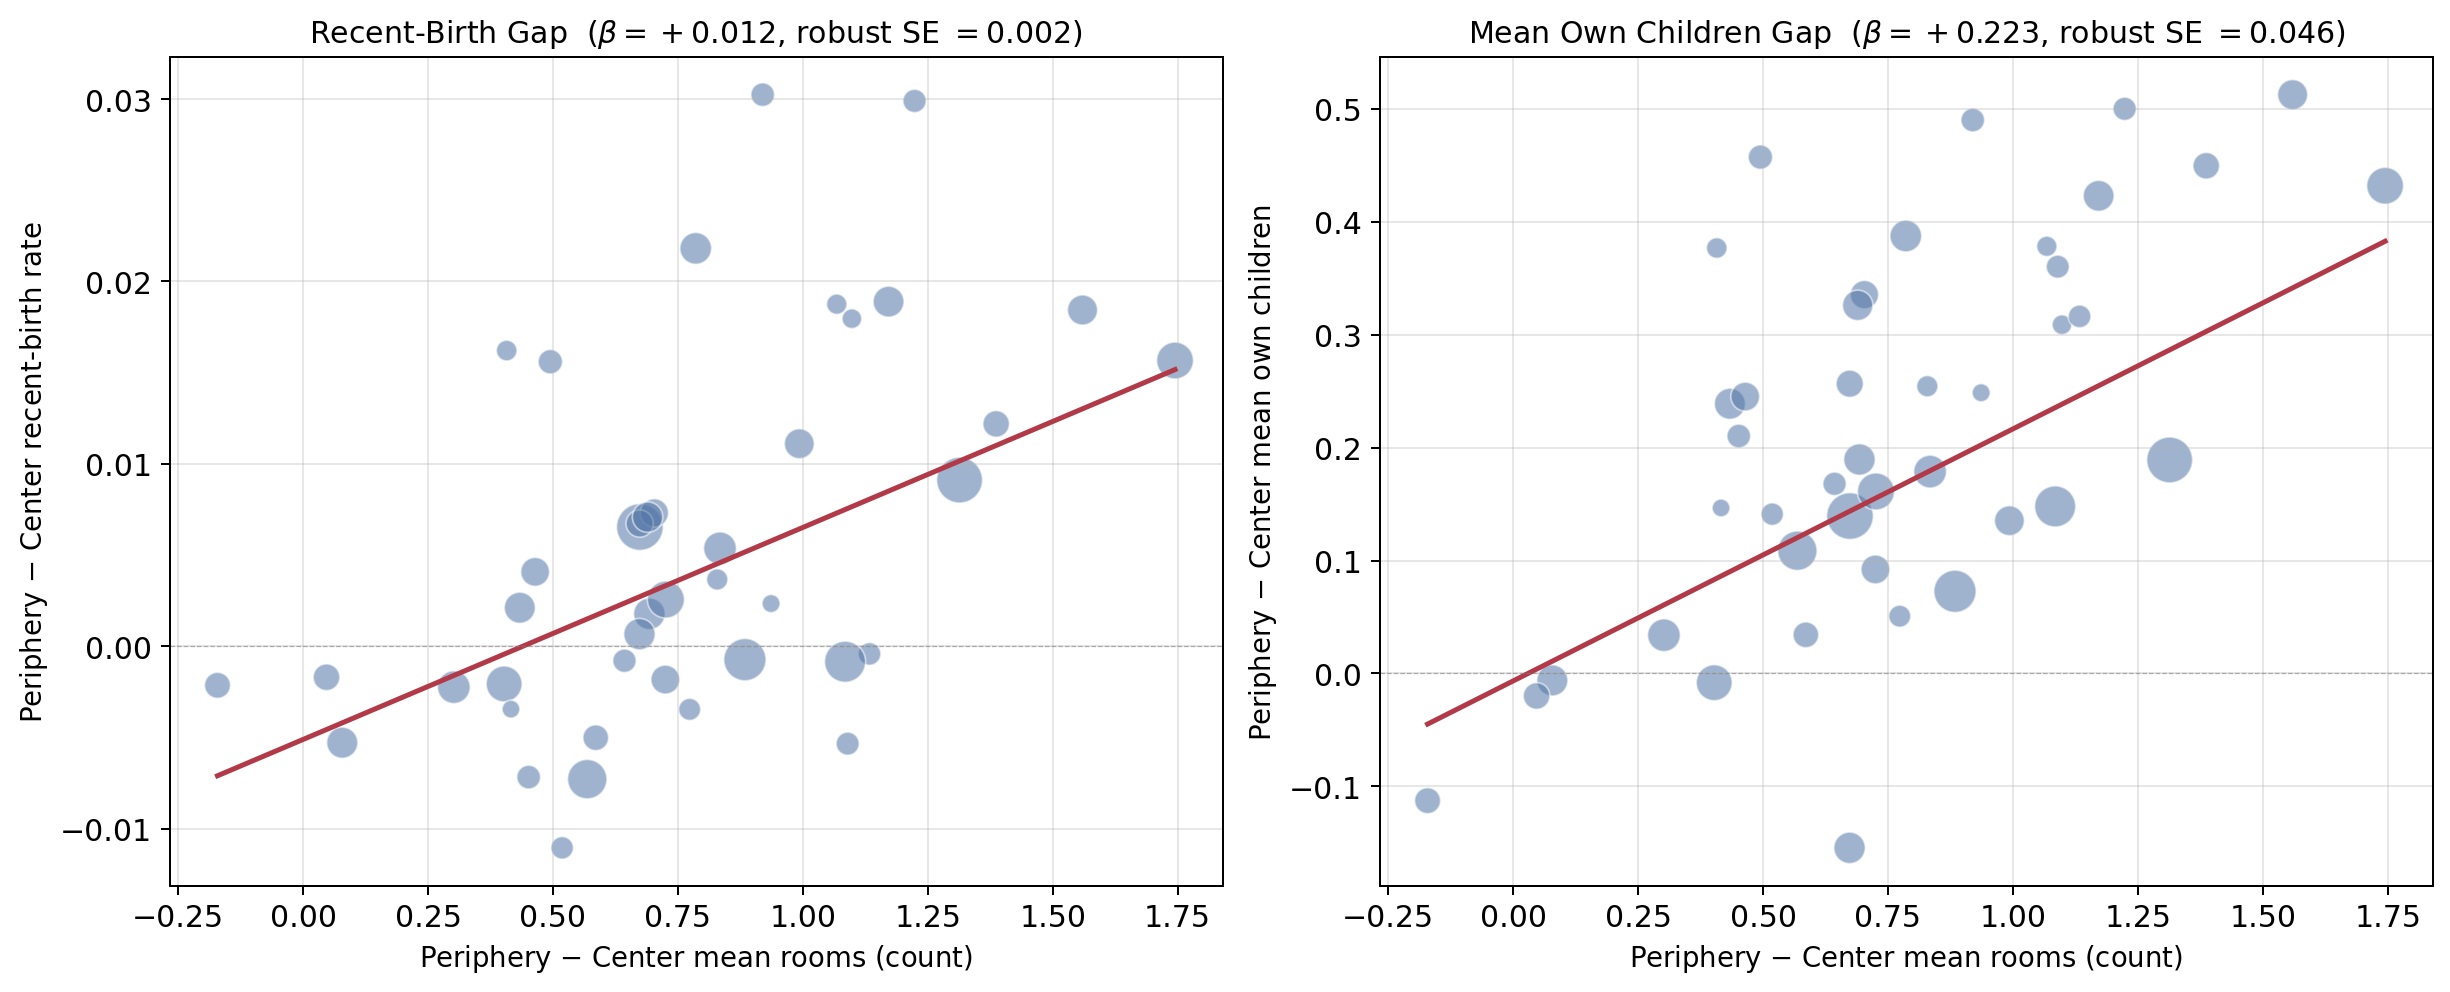
\includegraphics[height=0.58\textheight,trim=496 0 0 0,clip]{../docs/model/family_space_empirical_packet_2026-05-24/figures/rooms_gap_vs_fertility_gap.png}
\end{minipage}

\end{frame}

\begin{frame}{Big Units Are Owned}
\label{ahs_big_units_owned_body}
\centering
\includegraphics[width=0.72\linewidth,height=0.80\textheight,keepaspectratio]{../code/data/ahs_supply_snapshot/output_ahs_family_unit_menu_national/ahs_tenure_share_within_size.png}
\end{frame}

\begin{frame}{Using the PSID: Event-Study Design}
\small
For household $i$, let $E_i$ denote the year of childbirth. For any housing outcome $Y_{it}$, estimate
\[
Y_{it}
=
\sum_{k=-5,k\neq -2}^{10} \alpha_k \mathbf{1}\{t-E_i = k\}
+ \zeta_i + \tau_t + \delta X_{it} + \varepsilon_{it}.
\]
\begin{itemize}
  \item $\zeta_i$ and $\tau_t$ are household and calendar-year fixed effects.
  \item The omitted period is $k=-2$, so each $\alpha_k$ is relative to two years before birth.
  \item I use the same design for homeownership, moving-for-size, and rooms.
  \item Geocoded data analysis in progress.
\end{itemize}
\end{frame}

\begin{frame}{PSID: Childbirth Raises Moves for Space \; \hyperlink{psid_reasons_questionnaire}{\beamerbutton{Reasons}} \hyperlink{psid_ev_housing_reasons}{\beamerbutton{By Category}}}
\label{psid_moves_body}

{\small $\hat\alpha_k$: change in probability of moving for reason $Y$, relative to $k=-2$.}

\smallskip
\begin{columns}[T]
\begin{column}{0.48\textwidth}
\centering
{\footnotesize $Y = \mathbf{1}\{\text{moved for expansion of housing}\}$}

\smallskip
\includegraphics[width=\linewidth]{../../Outputs/Graphs/mv_s_f_c_y_all.png}
\end{column}
\begin{column}{0.48\textwidth}
\centering
{\footnotesize $Y = \mathbf{1}\{\text{moved for neighborhood quality}\}$}

\smallskip
\includegraphics[width=\linewidth]{../../Outputs/Graphs/mv_n_f_c_y_all.png}
\end{column}
\end{columns}

\medskip
\footnotesize
\begin{itemize}
  \item The probability of moving for housing size rises around first birth.
  \item By contrast, moves for neighborhood quality do not rise in the same way.
\end{itemize}
\end{frame}

\begin{frame}{PSID: Ownership and Housing Size Around First Birth \; \hyperlink{slide1-main}{\beamerbutton{Details}}}
\label{psid_own_body}
\label{psid_rooms_body}
{\small \textit{Model: $\bar h(1) > \bar h(0)$; kids raise ownership.} \quad $\hat\alpha_k$: change relative to $k=-2$.}

\smallskip
\begin{columns}[T]
\begin{column}{0.48\textwidth}
\centering
{\footnotesize $Y_{it} = \mathbf{1}\{\text{owner}\}_{it}$}

\smallskip
\includegraphics[width=\linewidth]{../../Outputs/Graphs/own_f_c_y_all.png}
\end{column}
\begin{column}{0.48\textwidth}
\centering
{\footnotesize $Y_{it} = \text{number of rooms}_{it}$}

\smallskip
\includegraphics[width=\linewidth]{../../Outputs/Graphs/rooms_f_c_y_all.png}
\end{column}
\end{columns}

\medskip
\footnotesize
\begin{itemize}
  \item Homeownership rises sharply after first birth; rooms expand by about 0.66 at $k=+3$.
\end{itemize}
\scriptsize Pre-birth mean: 6.0 rooms.
\end{frame}


\section{Quantification}

\begin{frame}[plain,c,noframenumbering]
\centering
{\Large\textbf{Quantification}}
\end{frame}

\begin{frame}{Externally Calibrated Parameters}
\small
\renewcommand{\arraystretch}{0.95}
\centering
\begin{tabular}{llclc}
\toprule
& \textbf{Param} & \textbf{Description} & \textbf{Value} & \textbf{Source} \\
\midrule
\textit{Pref.} & $\sigma$ & Risk aversion & 2.0 & -- \\
& $\bar c_0$ & Consumption floor & 0.10 & Poverty line \\
\midrule
\textit{Fin.} & $q$ & Gross bond rate & 1.04 & -- \\
& $\delta$ & Depreciation & 0.02 & Greaney et al.\ (2024) \\
& $\tau_H$ & Property tax & 0.01 & US average \\
& $\phi$ & LTV limit & 0.80 & 20\% down payment \\
& $\psi$ & Transaction cost & 0.06 & Greaney et al.\ (2024) \\
\midrule
\textit{Life} & $J$, $J_R$ & Lifespan, retirement & 60, 47 & Ages 18--77, ret.\ 65 \\
& $\tau_{\text{pay}}$ & Payroll tax & 0.179 & Greaney et al.\ (2024) \\
\midrule
\textit{Housing} & $\eta_P$, $\eta_C$ & Supply elasticities & 2.0, 0.8 & Saiz (2010) \\
\bottomrule
\end{tabular}
\end{frame}

\begin{frame}{Internally Calibrated Parameters \; \hyperlink{app:calibration_strategy}{\beamerbutton{Strategy}}}
\footnotesize
\renewcommand{\arraystretch}{0.85}
\centering
\begin{tabular}{llc}
\toprule
\textbf{Param} & \textbf{Description} & \textbf{Value} \\
\midrule
$\mathcal{E}_C$ & Center amenity & 0.140 \\
$\bar r_C$ & Center rent anchor & 0.096 \\
$\alpha$ & Consumption weight & 0.871 \\
$\beta$ & Discount factor & 0.953 \\
$b_0$ & Entry wealth & 0.398 \\
$\chi$ & Owner utility premium & 1.298 \\
$\psi_{\text{child}}$ & Flow utility of children & 0.071 \\
$\kappa_f$ & Fertility Gumbel scale & 3.816 \\
$\bar h_0$ & Baseline housing need & 3.231 \\
$\bar h_{\text{jump}}$ & Housing jump (1st child) & 0.986 \\
$\bar h_n$ & Add'l child housing cost & 0.548 \\
$\bar c_n$ & Add'l-child cons.\ cost & 0.110 \\
$\kappa_i$ & Location-choice Gumbel scale & 1.448 \\
$\mu_{\text{move}}$ & Moving cost & 4.140 \\
$\theta_0$ & Bequest shifter & 0.595 \\
$\theta_n$ & Bequest parent premium & 0.352 \\
\bottomrule
\end{tabular}
\end{frame}

\begin{frame}{Calibration Targets}
\small\fontsize{8.3}{9.6}\selectfont
\centering
\renewcommand{\arraystretch}{0.78}
\begin{tabular}{@{}llrr@{}}
\toprule
\textbf{} & \textbf{Moment} & \textbf{Target} & \textbf{Model} \\
\midrule
\textit{Fertility} & TFR & 1.700 & 1.770 \\
& Ever childless & 0.150 & 0.191 \\
& Age at first birth & 26.0 & 34.0 \\
& Fertility gradient $P{-}C$ & 0.133 & 0.166 \\
\midrule
\textit{Housing} & Ownership, ages 30--55 & 0.575 & 0.684 \\
& Ownership gradient $P{-}C$ & 0.186 & 0.107 \\
& $H_{01}$ (PSID, rooms) & 0.664 & 1.261 \\
& $H_{12}$ (PSID, rooms) & 0.566 & 0.379 \\
& Parent ownership gap & 0.168 & 0.185 \\
& Housing exp.\ share & 0.240 & 0.251 \\
\midrule
\textit{Saving} & Liq.\ wealth / income & 0.600 & 0.443 \\
\midrule
\textit{Location} & Center population share & 0.450 & 0.425 \\
& Rent/room ratio $C/P$ & 1.140 & 1.184 \\
& Center share, non-parents & 0.494 & 0.373 \\
& Center share, new parents & 0.416 & 0.361 \\
& C--P switching rate & 0.032 & 0.044 \\
\midrule
\textit{Bequest} & Ownership, ages 65--75 & 0.764 & 0.767 \\
& Parent--childless own gap & 0.070 & 0.036 \\
\bottomrule
\end{tabular}
\end{frame}

\begin{frame}{Lifecycle Fit \; \hyperlink{app:housing_fit}{\beamerbutton{Housing Fit}}}
\label{slide:lifecycle_fit}
\centering
\includegraphics[width=\textwidth,height=0.85\textheight,keepaspectratio]{../output/model/alpha_share_a24_w250_20260528_compare_job011_job001/alpha_a24_job011/figures/benchmark_lifecycle_compare.png}
\end{frame}

\begin{frame}{Spatial Lifecycle Fit \; \hyperlink{app:aggregate_full_wealth}{\beamerbutton{Aggregate Wealth}}}
\label{slide:spatial_lifecycle_fit}
\centering
\includegraphics[width=\textwidth,height=0.85\textheight,keepaspectratio]{../output/model/alpha_share_a24_w250_20260528_compare_job011_job001/alpha_a24_job011/figures/spatial_lifecycle_3x2_model_vs_data_lifetime.png}
\end{frame}

\begin{frame}{Equilibrium}
\centering
\includegraphics[width=\textwidth,height=0.85\textheight,keepaspectratio]{../output/model/alpha_share_a24_w250_20260528_compare_job011_job001/alpha_a24_job011/figures/market_equilibrium.png}
\end{frame}

\begin{frame}{Intergenerational Allocation: Model vs Data}
\label{acs_redfin_model_vs_data_body}
\centering
\includegraphics[width=0.92\linewidth,height=0.78\textheight,keepaspectratio]{../output/model/house_size_by_age_v1/big_homes_rooms_data_vs_model.png}

\smallskip
\scriptsize Owner-occupied units with $\geq 6$ rooms. Heads of household, ACS 2022--2023.
\end{frame}


\begin{frame}{Conclusion}
\begin{itemize}
  \item A model of fertility with realistic housing and lifecycle
  \item Trying to capture the many implications of children's impact on housing demand 
  \item Aim is policy. Want to increase fertility: Can housing help? What costs?
  \item More work is needed:
  \begin{itemize}
    \item Theory: important to understand the role of constraints and sorting incentives. Can we say something about policy design?
    \begin{itemize}
      \item Financial constraints
      \item Size supply and allocation of family space
    \end{itemize}
    \item Empirically: use new geocoded data to track location and moves
    \item Quantification: use the model to evaluate policies that target housing to parents, and understand the channels
  \end{itemize}
\end{itemize}
\end{frame}

\begin{frame}[plain,c,noframenumbering]
\centering
{\Large\textbf{Thank You}}
\end{frame}

\appendix

\begin{frame}[plain,c,noframenumbering]
\centering
{\Large\textbf{Appendix}}
\end{frame}

\begin{frame}{Appendix: Who Owns America's Large Homes? \; \hyperlink{acs_redfin_model_vs_data_body}{\beamerbutton{Back}}}
\label{acs_redfin_replica_body}
\centering
\includegraphics[width=0.78\linewidth,height=0.78\textheight,keepaspectratio]{../code/data/mms_center_periphery/output_redfin_big_homes_replica/redfin_big_homes_replica.png}

\smallskip
\scriptsize ACS 2022--2023, household heads, owner-occupied $3{+}$ bedroom units. Generations defined by birth year. ``With own children'' uses youngest-child age $<18$.
\end{frame}

\begin{frame}{Appendix: PSID -- Wealth Gate on Childlessness}
\label{app:wealth_gate_body}
\footnotesize
\textbf{Shortfall:} renter's liquid wealth $<\,0.035 \times P^{\text{target}}_t$, where $P^{\text{target}}_t$ is the median first-time-buyer home value (the FHA $3.5\%$ DP floor).

\smallskip
\centering
\includegraphics[width=0.62\linewidth,height=0.55\textheight,keepaspectratio]{../code/data/psid_followup_mar2026/output/dp_shortfall_v1/childless_by_shortfall_inc_tercile_v1.png}

\smallskip
\scriptsize
PSID renters $25$--$30$, pre-first-birth, $N=2{,}961$. Shortfall renters are $8.8$ pp more childless by $45$, controlling for $\log$ income and $\log$ NW ($p=0.003$).
\end{frame}

\begin{frame}{Appendix: PSID -- Wealth Gate Works Through Large Homes}
\label{app:hacamo_replica_body}
\footnotesize
\textbf{Shortfall:} as defined on previous slide.\quad
\textbf{Joint:} $\mathbf{1}\{\text{first purchase by } 40 \cap \text{first birth by } 40\}$, split by home size at purchase.

\smallskip
\centering
\begin{tabular}{lccc}
\toprule
 & (1) & (2) & (3) \\
 & joint, any & joint, large & joint, small \\
 & & ($\geq 4$ rooms) & ($<4$ rooms) \\
\midrule
Shortfall          & $-0.097^{**}$ & $-0.092^{*}$ & $-0.005$  \\
                   & $(0.047)$     & $(0.047)$    & $(0.014)$ \\
\addlinespace
$\log$ income      & $0.100^{***}$ & $0.112^{***}$ & $-0.012$  \\
                   & $(0.022)$     & $(0.021)$    & $(0.009)$ \\
\addlinespace
$\log$ net worth   & $-0.007$      & $-0.007$     & $0.000$   \\
                   & $(0.005)$     & $(0.005)$    & $(0.001)$ \\
\midrule
Observations       & $1{,}554$     & $1{,}554$    & $1{,}554$ \\
$R^2$              & $0.031$       & $0.035$      & $0.003$   \\
\bottomrule
\end{tabular}

\smallskip
\scriptsize PSID renters $25$--$30$, pre-first-birth, followed to $40$. PSID weights, robust SE in parentheses. $^{*}p<0.10$, $^{**}p<0.05$, $^{***}p<0.01$.
\end{frame}

% ==================================================================
% Theory block: Lemma 2 (sorting), Lemma 3 (constrained squeeze).
% ==================================================================

\begin{frame}{Appendix: Sorting and Housing-Demand Elasticity}
\label{slide1-main}

\footnotesize

$\mathcal E_C > \mathcal E_P$ (amenity); $r_C > r_P$ (rents); $M = qb + y - b'$ (expenditure budget);\\ $\bar h(n)$ housing requirement with $n$ children, $\bar h(1) > \bar h(0)$. Ignoring moving costs and Gumbel

\vspace{0.3em}
\textbf{Sorting.}
\begin{itemize}\setlength\itemsep{1pt}
  \item Higher $\bar h$ $\Rightarrow$ larger rent bill in $C$ $\Rightarrow$ preference for $C$ falls.
  \item Single crossing: for each $M$, unique threshold $\hat h(M)$ s.t.\ $\bar h < \hat h \Rightarrow C$,\; $\bar h > \hat h \Rightarrow P$.
  \item $\hat h$ rises with $M$ (richer households absorb high $r_C$).
  \item Since $\bar h(1) > \bar h(0)$: parents sort weakly peripheral.
  \begin{itemize}\scriptsize
    \item Parent share falls with local rent.
    \item First birth triggers moves to lower-$r$ areas.
  \end{itemize}
\end{itemize}

\vspace{0.2em}
\textbf{Elasticity.}\;
Housing demand for uncapped renter splits into committed $+$ discretionary:
\vspace{-0.5em}
\[
h^\ast(n) = \underbrace{\alpha\,\bar h(n)}_{\text{committed}} + \underbrace{\tfrac{(1-\alpha)(M-\bar c)}{r}}_{\text{discretionary}}.
\]
\vspace{-0.8em}
  \begin{itemize}\scriptsize
    \item Parents less income-elastic on intensive margin; less responsive to rent.
    \item Kids raise the probability of owning.
  \end{itemize}

\end{frame}

\begin{frame}{Appendix: Sorting and Rents \; \hyperlink{acs_sorting_family_space_body}{\beamerbutton{Back}}}
\label{slide2-main}

\setbeamerfont{block title}{size=\footnotesize}
\footnotesize
\begin{itemize}
\item In this static derivation, let $\mathcal V_i(n;M)$ be indirect utility
for a renter with $n$ children in location $i$.
\item $\Delta\mathcal V(n;M)\equiv \mathcal V_C(n;M)-\mathcal V_P(n;M)$
\item Sorting wedge: $\mathcal W(M)\equiv\Delta\mathcal V(0;M)-\Delta\mathcal V(1;M)>0$
\item If the rent gap $r_C - r_P$ widens, the parent-childless gap in location preferences $\mathcal W$ widens:
\[
\left.\frac{\partial \mathcal W}{\partial r_C}\right|_{r_P} > 0.
\]
\end{itemize}

\begin{itemize}\setlength\itemsep{-1pt}
  \item Across cities: the parent-childless center-share gap rises with the local center-periphery rent gap.
\end{itemize}

\end{frame}

\begin{frame}{Appendix: Constrained Squeeze \; \hyperlink{app:lem3-cev}{\beamerbutton{derivation}}}
\label{lem3-main}

\footnotesize

Capped renters and owners on a fixed rung cannot adjust housing. How costly is a child on a home that barely fits one?

\vspace{0.2em}
Consumption-equivalent variation, holding housing fixed:
\vspace{-0.4em}
\[
u(c + \mathrm{CEV},\; h,\; 1) \;=\; u(c,\; h,\; 0).
\]
\vspace{-0.6em}
	Pre-birth slack $s^0 = h - \bar h(0)$ and extra required space
	$\Delta\bar h=\bar h(1)-\bar h(0)$.

\vspace{0.2em}
\centering
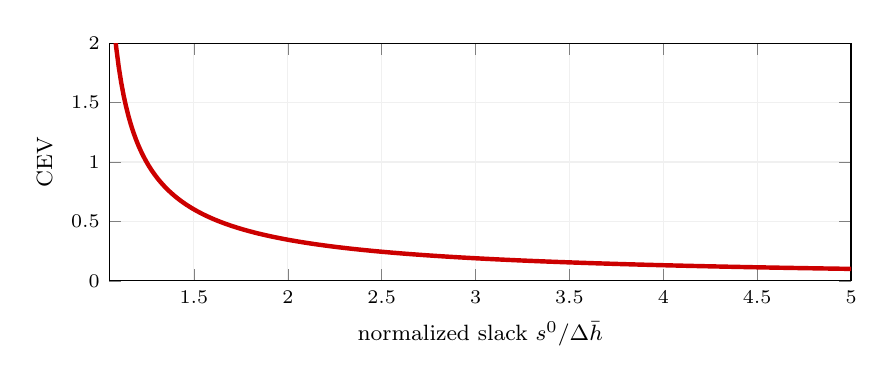
\begin{tikzpicture}
\begin{axis}[
  width=11cm, height=4.6cm,
	  xlabel={\footnotesize normalized slack $s^0/\Delta\bar h$},
  ylabel={\footnotesize CEV},
  xmin=1.05, xmax=5.0, ymin=0, ymax=2.0,
  samples=300, domain=1.06:5.0,
  grid=both, grid style={gray!12},
  tick label style={font=\scriptsize}, label style={font=\footnotesize}
]
  \addplot[ultra thick, red!80!black] {(x/(x-1))^(3/7)-1};
	  \draw[gray, dashed, thick] (axis cs:1.0,0) -- (axis cs:1.0,2.0)
	    node[above, font=\scriptsize] {$s^0 = \Delta\bar h$};
\end{axis}
\end{tikzpicture}
\end{frame}


\begin{frame}[t]{Appendix: Entry Shares and City-Entry Probability \; \hyperlink{slide:entry_stationarity}{\beamerbutton{Back}}}
\label{app:entry_shares_probs}
\footnotesize
\setlength{\abovedisplayskip}{3pt}\setlength{\belowdisplayskip}{3pt}

\begin{itemize}\setlength\itemsep{4pt}
  \item Potential entrant draws EV-I tastes over $\{C, P, \text{outside}\}$ with scale $\kappa_E$
  \item Modeled-location values $W_C^E$, $W_P^E$ (from solving as childless renters at $(b^E, R, i, 0, 0, 0)$); outside value $\bar W^E$
  \item Logit shares:
  \[
  \pi_i^E=\frac{\exp(W_i^E/\kappa_E)}{\exp(W_C^E/\kappa_E)+\exp(W_P^E/\kappa_E)+\exp(\bar W^E/\kappa_E)},
  \quad i\in\{C,P\}
  \]
  \[
  \pi_{\mathrm{out}}^E=\frac{\exp(\bar W^E/\kappa_E)}{\exp(W_C^E/\kappa_E)+\exp(W_P^E/\kappa_E)+\exp(\bar W^E/\kappa_E)}
  \]
  \item Sum to one: $\pi_C^E+\pi_P^E+\pi_{\mathrm{out}}^E=1$
  \item \textbf{City entry probability}: $q^E=\pi_C^E+\pi_P^E=1-\pi_{\mathrm{out}}^E$
  \item $\pi_i^E$ determines \emph{where} entrants go inside the city; $q^E$ determines \emph{how many} enter
\end{itemize}
\end{frame}

\begin{frame}[t]{Appendix: Entry Accounting Algorithm \; \hyperlink{slide:entry_stationarity}{\beamerbutton{Back}}}
\label{app:entry_accounting}
\scriptsize
\setlength{\abovedisplayskip}{3pt}\setlength{\belowdisplayskip}{3pt}
\begin{enumerate}\setlength\itemsep{4pt}
  \item Solve the benchmark in normalized units: $S^*=1$. The normalized
  composition gives $E_{0C}^*$, $E_{0P}^*$, $E_0^*=E_{0C}^*+E_{0P}^*$, and $B_0^*$.

  \item Pick the benchmark outside margin. Choose $\bar W^E$ so that entry
  probabilities satisfy
  \[
  q^{E,*}=\pi_C^{E,*}+\pi_P^{E,*}.
  \]

  \item Use the aggregate stationarity equation at $S^*=1$ to recover the
  outside-origin potential entrant mass:
  \[
  M=\frac{E_0^*}{q^{E,*}}-B_0^*.
  \]

  \item The solve must also reproduce entry by location:
  \[
  S E_{0i}=\left[M+S B_0\right]\pi_i^E,\qquad i\in\{C,P\}.
  \]
  The scalar equation for $S$ is the sum of these two conditions.

  \item In counterfactuals, keep $(M,\bar W^E,\kappa_E)$ fixed. Recompute
  household values, $E_0$, $B_0$, and $q^E$, then set
  \[
  S=\frac{q^E M}{E_0-q^E B_0},
  \qquad
  E_i=\left[M+S B_0\right]\pi_i^E.
  \]
\end{enumerate}
\end{frame}

\begin{frame}[t]{Appendix: Distributional Stationarity}
\footnotesize
\setlength{\abovedisplayskip}{4pt}\setlength{\belowdisplayskip}{4pt}
\begin{itemize}\setlength\itemsep{6pt}
  \item The stationary object is the normalized composition $g$ together with
  city scale $S$. The level mass of any household state is $Sg$.

  \item Incumbent households transition through policies, fertility, location
  choice, aging, and death.

  \item Location-specific entrant masses are
  \[
  E_i=\left[M+S B_0\right]\pi_i^E,
  \qquad i\in\{C,P\}.
  \]
  These entrants are placed at the entrant states $x_i^E$.

  \item The scalar equation for $S$ is only the sum of the two entry-location
  equations. The equilibrium still has to reproduce the location distribution
  inside $g$.
\end{itemize}
\end{frame}

\begin{frame}{Calibration Strategy}
\label{app:calibration_strategy}
\footnotesize
\begin{columns}[T,onlytextwidth]
\begin{column}{0.48\textwidth}
\textbf{Externally set}
\begin{itemize}\setlength\itemsep{-1pt}
  \item Lifecycle structure, taxes, interest rate
  \item Collateral ($\phi=0.80$), transaction cost ($\psi=0.06$)
  \item Housing ladder and supply elasticities
\end{itemize}
\end{column}
\begin{column}{0.48\textwidth}
\textbf{Internally calibrated (SMM)}
\begin{itemize}\setlength\itemsep{-1pt}
  \item 15 parameters: 2 inverted (amenity, rent anchor) + 13 searched
  \item Fertility, tenure, mobility, saving, bequests
  \item 17 target moments from ACS and PSID
\end{itemize}
\end{column}
\end{columns}

\medskip
\begin{itemize}\setlength\itemsep{-1pt}
  \item Five owner sizes at $\{5.2, 5.85, 6.55, 7.55, 9.0\}$ rooms; rental cap at 4.8 rooms.
  \item Bequests parameterized by $(\theta_0,\theta_n)$ with fixed $\theta_1=0.01$.
\end{itemize}
\end{frame}

% ==================================================================
% Appendix slides for the simple-spatial theory block
% ==================================================================

% ----- Appendix setup: utility, demands, indirect utility -----
\begin{frame}{Appendix: Setup --- Utility, Demands, Indirect Utility \; \hyperlink{slide1-main}{\beamerbutton{back}}}
\label{app:setup}
\small

Common preliminaries for the derivations that follow.

\vspace{0.4em}
\textbf{Utility} (CRRA over Cobb--Douglas Stone--Geary):
\vspace{-0.4em}
\[
u(c,h;m) = \frac{\bigl[(c-\bar c(m))^\alpha(h-\bar h(m))^{1-\alpha}\bigr]^{1-\sigma}}{1-\sigma}.
\]

\vspace{0.2em}
\textbf{Interior demands} ($\sigma$-invariant). With $M$ household resources, rent $r_i$ in location $i$, and $\tilde M_i(\bar h) = M - \bar c - r_i\bar h$:
\vspace{-0.4em}
\[
c^\ast - \bar c = \alpha\,\tilde M_i,
\qquad
h^\ast - \bar h = (1-\alpha)\,\tilde M_i / r_i.
\]

\vspace{0.2em}
\textbf{Indirect utility with amenity $\mathcal E_i$:}
\vspace{-0.4em}
\[
\mathcal V_i(\bar h; M) = \frac{Z^\ast(\bar h; M, r_i)^{1-\sigma}}{1-\sigma} + \mathcal E_i,
\quad
Z^\ast = \alpha^\alpha(1-\alpha)^{1-\alpha}\,\tilde M_i\,r_i^{-(1-\alpha)}.
\]
\end{frame}

\begin{frame}{Appendix: Sorting Derivation \; \hyperlink{slide1-main}{\beamerbutton{back}}}
\label{app:sorting}
\small

For $r_C > r_P$, $\mathcal E_C > \mathcal E_P$, define
$\Delta\mathcal V(\bar h;M)=\mathcal V_C(\bar h;M)-\mathcal V_P(\bar h;M)$.

\vspace{0.4em}
\textbf{Derivative.} With $\gamma \equiv \alpha + \sigma(1-\alpha) > 0$ and
$\kappa \equiv \alpha^\alpha (1-\alpha)^{1-\alpha}$,
\[
\frac{d\,\Delta\mathcal V}{d\bar h}
= -\,\kappa^{1-\sigma}\!\left[\frac{r_C^{\gamma}}{\tilde M_C^{\sigma}}
  - \frac{r_P^{\gamma}}{\tilde M_P^{\sigma}}\right] < 0.
\]

\vspace{0.3em}
\textbf{Sign.} $r_C > r_P$ implies $r_C^\gamma > r_P^\gamma$;
$\tilde M_C < \tilde M_P$ implies $\tilde M_C^{-\sigma} > \tilde M_P^{-\sigma}$.
Both factors favour $C$, so the bracket is strictly positive and the
derivative is strictly negative.

\vspace{0.4em}
\textbf{Threshold.} Since $\Delta\mathcal V$ is continuous and strictly
decreasing in $\bar h$, the equation $\Delta\mathcal V(\hat h;M) = 0$
has at most one solution. Existence on a non-degenerate interval
follows from $\Delta\mathcal V(0;M)>0$ (amenity-positive) and
$\Delta\mathcal V(\bar h;M)\to-\infty$
as $\bar h \uparrow (M-\bar c)/r_C$ (infeasibility in $C$). Unique
threshold $\hat h(M)$.

\vspace{0.4em}
\textbf{Parent--childless ordering.} $\bar h(1) > \bar h(0)$ and $\Delta\mathcal V$
strictly decreasing $\Rightarrow$ parents weakly prefer the periphery,
strictly when $\bar h(0) < \hat h(M) < \bar h(1)$.
\end{frame}

\begin{frame}{Appendix: Elasticity-Attenuation Derivation \; \hyperlink{slide1-main}{\beamerbutton{back}}}
\label{app:elasticity}
\footnotesize

\textbf{Simplified demand} (interior renter at rent $r$; assume $\bar c(0)=\bar c(1)=\bar c$ so that only the housing requirement varies with the number of children):
\[
h^\ast(n) = \alpha\,\bar h(n) + (1-\alpha)\,\frac{M-\bar c}{r}.
\]

\vspace{0.4em}
\textbf{Elasticities.}
\[
e_M(n) = \frac{\partial \log h^\ast}{\partial \log M}
= \frac{(1-\alpha)(M-\bar c)}{r\,h^\ast(n)},
\qquad
e_r(n) = \frac{\partial \log h^\ast}{\partial \log r}
= -\,\frac{(1-\alpha)(M-\bar c)}{r\,h^\ast(n)}.
\]

\vspace{0.4em}
\textbf{Attenuation.} $h^\ast(n)$ is strictly increasing in $\bar h(n)$
(coefficient $\alpha > 0$); the numerator is independent of $\bar h(n)$.
Hence both $e_M(n)$ and $|e_r(n)|$ are strictly decreasing in
$\bar h(n)$. Since $\bar h(1) > \bar h(0)$:
\[
e_M(1) < e_M(0),
\qquad
|e_r(1)| < |e_r(0)|.
\]

\vspace{0.4em}
\textbf{Limits.} As $\bar h \to 0$, both elasticities $\to \mp 1$
(Cobb--Douglas benchmark). As $\bar h \to (M-\bar c)/r$ (feasibility
boundary), both $\to 0$ (pure subsistence).

\vspace{0.4em}
\textbf{Identification.} The gap $e_M(0) - e_M(1) > 0$ pins down
	$\Delta\bar h = \bar h(1) - \bar h(0)$ given $\alpha$, $M-\bar c$, and $r$.
\end{frame}

\begin{frame}{Appendix: Cross-Metro Sorting-Wedge Derivation \; \hyperlink{slide2-main}{\beamerbutton{back}}}
\label{app:wealth}
\footnotesize

Indirect utility on an interior renter branch in location $i$ with $n$ children ($\sigma=1$ for transparency; signs go through for any $\sigma > 0$):
\[
\mathcal V_i(n;M) = \log \tilde M_i^n - (1-\alpha)\log r_i + \mathcal E_i,
\quad
\tilde M_i^n = M - \bar c(n) - r_i \bar h(n).
\]

\vspace{0.4em}
\textbf{Sorting wedge.} Define
$\Delta\mathcal V(n;M)=\mathcal V_C(n;M)-\mathcal V_P(n;M)$ and
$\mathcal W(M)\equiv\Delta\mathcal V(0;M)-\Delta\mathcal V(1;M)$:
\[
\mathcal W(M) = \log\frac{\tilde M_C^0\,\tilde M_P^1}{\tilde M_C^1\,\tilde M_P^0}.
\]

\vspace{0.4em}
\textbf{Comparative statics in rents.} Using $\partial \tilde M_i^n/\partial r_i = -\bar h(n)$,
\[
\frac{\partial \mathcal W}{\partial r_C}
= \frac{\delta_h(M-\bar c(0)) + \bar h(0)\,\delta_c}{\tilde M_C^1\,\tilde M_C^0} > 0,
\qquad
\frac{\partial \mathcal W}{\partial r_P}
= -\frac{\delta_h(M-\bar c(0)) + \bar h(0)\,\delta_c}{\tilde M_P^1\,\tilde M_P^0} < 0.
\]
Numerators positive by interior feasibility ($M > \bar c(0)$) plus $\delta_c, \delta_h, \bar h(0) > 0$; denominators positive on the interior renter branch.

\vspace{0.4em}
\textbf{Reading.} Raising the centre rent (or lowering the periphery rent) widens the parent--childless sorting wedge: the cross-metro elasticity of sorting strength to the local rent gap is strictly positive. Same algebraic structure carries through for capped renters (replace $\tilde M_i^n$ with $\check M_i^n = M - r_i \bar h_R - \bar c(n)$).
\end{frame}

\begin{frame}{Appendix: Constrained-Squeeze CEV Derivation \; \hyperlink{lem3-main}{\beamerbutton{back}}}
\label{app:lem3-cev}
\small

	CEV solves $u(c,h,0) = u(c+\mathrm{CEV}, h, 1)$: housing quantity is
	held fixed at $h$, and the post-child surplus shrinks via
	$\bar h(n)$ from $s^0 = h - \bar h(0)$ to
	$s^0-\Delta\bar h = h - \bar h(1)$.
Under Stone--Geary
$u = [(c-\bar c(n))^\alpha(h-\bar h(n))^{1-\alpha}]^{1-\sigma}/(1-\sigma)$
and $\bar c(0) = \bar c(1) = \bar c$, equating utilities:
\[
(c - \bar c)^\alpha\, (s^0)^{1-\alpha}
	= (c + \mathrm{CEV} - \bar c)^\alpha\, (s^0-\Delta\bar h)^{1-\alpha}.
\]
Rearrange:
\[
\frac{c + \mathrm{CEV} - \bar c}{c - \bar c}
	= \left(\frac{s^0}{s^0-\Delta\bar h}\right)^{\!(1-\alpha)/\alpha}
	\;\Longrightarrow\;
	\mathrm{CEV} = (c - \bar c)\!\left[\!\left(\tfrac{s^0}{s^0-\Delta\bar h}\right)^{\!(1-\alpha)/\alpha}\!\!-1\right].
\]

\end{frame}

\begin{frame}{Ownership Is the Binding Constraint on Fertility \; \hyperlink{transition_bar}{\beamerbutton{Aggregate Gap}}}
\label{within_wealth_gap_body}
\begin{columns}[T]
\begin{column}{0.58\textwidth}
\centering
\includegraphics[width=\linewidth]{../code/data/psid_followup_mar2026/output/fertility_wealth_v1/within_wealth_gap_v9.png}
\end{column}
\begin{column}{0.40\textwidth}
\small
Sample: PSID renters at ages 25--30, pre-first-birth, followed to age 45 ($N=1{,}127$).
\medskip
\begin{itemize}
  \item At \textbf{every} wealth quintile, renters who transition to ownership by 35 are 20--35 pp less likely to remain childless by 45.
  \item The gap does not shrink with wealth: even wealthy renters who do not buy remain ${\sim}55\%$ childless.
  \item Mediation regression: wealth has \textbf{zero} direct effect on fertility ($p=0.92$); the entire effect runs through ownership ($\beta=0.32$, $p<0.001$).
\end{itemize}
\end{column}
\end{columns}

\medskip
\footnotesize Quintiles of net worth / income at 25--30. Tenure transition: modal tenure at 31--35. Childlessness by age 45 from reported first-birth year.
\end{frame}

\begin{frame}{Wealth and Fertility: Two Channels}
\begin{columns}[T]
\begin{column}{0.58\textwidth}
\centering
\includegraphics[width=\linewidth]{../code/data/psid_followup_mar2026/output/fertility_wealth_v1/lpoly_parenthood_v12.png}
\end{column}
\begin{column}{0.40\textwidth}
\small
The unconditional wealth--fertility relationship is \textbf{hump-shaped}:
\medskip
\begin{itemize}
  \item \textbf{Rising part} (NW $<$ \$80k): more wealth $\Rightarrow$ can clear down payment $\Rightarrow$ access family-sized housing $\Rightarrow$ have children. The \emph{resource/housing channel}.
  \item \textbf{Falling part} (NW $>$ \$80k): wealthier young adults are disproportionately high human capital and career-invested. The \emph{opportunity cost channel}.
\end{itemize}

\medskip
The non-monotonicity is why we need a structural model: the housing channel cannot be read off the raw data.
\end{column}
\end{columns}

\medskip
\footnotesize PSID 1984--2019, all young adults at 25--30. Local linear smooth (Epanechnikov kernel, bw = \$25k). Trimmed at p2/p98.
\end{frame}

\begin{frame}{Aggregate Ownership Transition Gap \; \hyperlink{within_wealth_gap_body}{\beamerbutton{Back}}}
\label{transition_bar}
\begin{columns}[T]
\begin{column}{0.58\textwidth}
\centering
\includegraphics[width=\linewidth]{../code/data/psid_followup_mar2026/output/fertility_wealth_v1/childless_by_transition_v7_bar.png}
\end{column}
\begin{column}{0.40\textwidth}
\small
Among renters at 25--30 who have not yet had a first child:
\medskip
\begin{itemize}
  \item Those who transition to ownership by 35: \textbf{28\%} childless at 45.
  \item Those who stay renters through 35: \textbf{60\%} childless at 45.
  \item A \textbf{32 pp} extensive-margin gap---larger than any within-tenure wealth effect.
\end{itemize}
\end{column}
\end{columns}

\medskip
\footnotesize Tenure status averaged over ages 25--30 (renter) and 31--35 (transition outcome). Childlessness measured by 45 using reported age at first birth.
\end{frame}

\begin{frame}{PSID: Housing Also Expands After Second Birth \; \hyperlink{psid_rooms_body}{\beamerbutton{Back}}}
\centering
\includegraphics[width=0.78\textwidth,height=0.76\textheight,keepaspectratio]{../code/data/psid_followup_mar2026/output/sa_rooms_second_birth_with_onechild_controls_v1/rooms_s_c_y_all.png}

\medskip
\footnotesize Baseline second-birth event study with stay-at-one-child controls: the $+3$ coefficient is about \textbf{0.57 rooms}.
\end{frame}

\begin{frame}{PSID: Income Trajectories, Movers vs Non-Movers}
\label{psid_income_body}
\centering
\includegraphics[width=0.78\textwidth,height=0.76\textheight,keepaspectratio]{../../Outputs/Graphs/log_INCFAMFRmvr_vsn_mvr_f_c_y.png}
\end{frame}

\begin{frame}{Defining Center and Periphery Within Large Metros \; \hyperlink{cross_section_body}{\beamerbutton{Back}}}
\label{geography_def}
\footnotesize
\begin{itemize}\setlength\itemsep{0.7em}
  \item 51 metros with year-2000 population above 1 million.
  \item Rank tracts by distance to the CBD; the core is the closest 10\% of metro population.
  \item Aggregate tracts to PUMAs via centroids and tract population.
  \item PUMA is \emph{center} if $\geq 50\%$ of its population sits in core tracts, \emph{periphery} if $<10\%$, \emph{middle} otherwise.
  \item Binary split: middle PUMAs go to center. Center share: 45\%.
\end{itemize}

\vfill
\scriptsize Source: ACS 2012--2023, PUMA-level.
\end{frame}

\begin{frame}{Most Adjustment Is Within Metros \; \hyperlink{movers_body}{\beamerbutton{Back}}}
\label{app:within_moves}
\centering
\includegraphics[width=0.75\linewidth,trim=0 0 0 11mm,clip]{../code/data/mms_center_periphery/output_middle_center/mms_grouped_4way_decomposition_allparent.png}

\medskip
\begin{itemize}
  \item Most adjustment happens \textbf{within} metros rather than across metros.
\end{itemize}
\end{frame}

\begin{frame}{Mover Regressions: Parent vs.\ Non-Parent \; \hyperlink{movers_body}{\beamerbutton{Back}}}
\label{mover_regressions}
\begin{table}[htbp]\centering
\scriptsize
\begin{tabular}{l*{2}{c}}
\toprule
 & \multicolumn{1}{c}{(1)} & \multicolumn{1}{c}{(2)} \\
Outcome (pp) & New Parent & Any Parent \\
\midrule
Across-CBSA move                        & $-4.56\sym{***}$ & $-5.17\sym{***}$ \\
                                        & $(0.78)$ & $(0.54)$ \\
Center destination $\mid$ within-CBSA   & $-11.21\sym{***}$ & $-11.44\sym{***}$ \\
                                        & $(0.66)$ & $(0.53)$ \\
Within CBSA $\to$ Center                & $-6.77\sym{***}$ & $-6.79\sym{***}$ \\
                                        & $(0.77)$ & $(0.65)$ \\
Within CBSA $\to$ Periphery             & $11.33\sym{***}$ & $11.95\sym{***}$ \\
                                        & $(0.49)$ & $(0.30)$ \\
Center dest.\ $\mid$ center origin      & $-9.69\sym{***}$ & $-8.91\sym{***}$ \\
                                        & $(0.81)$ & $(0.53)$ \\
Center dest.\ $\mid$ periphery origin   & $-10.71\sym{***}$ & $-11.32\sym{***}$ \\
                                        & $(0.51)$ & $(0.47)$ \\
\midrule
Age and year FE                         & Yes & Yes \\
Sex and race controls                   & Yes & Yes \\
\bottomrule
\end{tabular}
\end{table}
\vspace{-0.8em}
\begin{flushleft}\tiny
\textit{Notes.} OLS on ACS 2012--2023 within-metro movers, ages 22--45, weighted by \texttt{perwt}. Coefficients in percentage points. Column (1) uses a \emph{new-parent} indicator (eldest child $<4$); column (2) uses an \emph{any-parent} indicator. Standard errors in parentheses. \sym{*}~$p<0.10$, \sym{**}~$p<0.05$, \sym{***}~$p<0.01$.
\end{flushleft}
\end{frame}

\begin{frame}{Cross-Metro Sorting Regression \; \hyperlink{acs_sorting_family_space_body}{\beamerbutton{Back}}}
\label{acs_crossmetro_reg}
\begin{table}[htbp]\centering
\scriptsize
\begin{tabular}{lcc}
\toprule
Dependent gap (pp) & Slope on log rent gap & Metros \\
\midrule
Center-share gap & $6.23$ & $42$ \\
                 & $(5.19)$ &  \\
Center-destination gap $\mid$ within-CBSA movers & $23.53\sym{***}$ & $42$ \\
                 & $(6.18)$ &  \\
\bottomrule
\end{tabular}
\end{table}
\vspace{-0.7em}
\begin{flushleft}\tiny
\textit{Notes.} Unit of observation is the metro. Each dependent variable is the non-parent minus new-parent gap in percentage points. Regressor is the local log center--periphery rent-per-room gap. Each regression is weighted by its corresponding metro sample size. \sym{***}~$p<0.01$.
\end{flushleft}
\end{frame}

\begin{frame}{Housing Demand Elasticity Among Renters \; \hyperlink{acs_sorting_family_space_body}{\beamerbutton{Back}} \hyperlink{acs_elasticity_reg}{\beamerbutton{Regression}}}
\label{acs_elasticity_body}
\footnotesize
\textit{Model: parents less income-elastic in housing ($\bar h(1) > \bar h(0)$).}
\centering
\includegraphics[width=0.60\linewidth]{../output/model/acs_supporting_facts_v1/acs_renter_rooms_elasticity_bars_v1.png}

\vspace{-0.2em}
\begin{center}
\scriptsize Mean rooms among renters: 4.20 for childless households, 4.92 for parents.
\end{center}
\vspace{-0.2em}
\begin{itemize}
  \item Parent renters start from a larger space baseline, but rooms rise less with income: elasticity 0.102 for parents versus 0.129 for childless renters.
\end{itemize}
\end{frame}

\begin{frame}{Renter Housing-Demand Elasticity \; \hyperlink{acs_elasticity_body}{\beamerbutton{Back}}}
\label{acs_elasticity_reg}
\begin{table}[htbp]\centering
\scriptsize
\begin{tabular}{lccc}
\toprule
Outcome & Childless slope & Parent interaction & Parent slope \\
\midrule
Log rooms & $0.129\sym{***}$ & $-0.027\sym{***}$ & $0.102\sym{***}$ \\
          & $(0.001)$ & $(0.001)$ & $(0.001)$ \\
\midrule
Metro FE & Yes & Yes & Yes \\
Age and year FE & Yes & Yes & Yes \\
Sex and race controls & Yes & Yes & Yes \\
Observations & \multicolumn{3}{c}{$3{,}024{,}081$} \\
\bottomrule
\end{tabular}
\end{table}
\vspace{-0.7em}
\begin{flushleft}\tiny
\textit{Notes.} OLS on ACS renters, ages 22--45, 2012--2023, weighted by \texttt{perwt}. Specification is $\log(\text{rooms})$ on $\log(\text{income})$, parent status, and the interaction, with metro, age, and year fixed effects plus sex and race controls. Standard errors in parentheses. \sym{***}~$p<0.01$.
\end{flushleft}
\end{frame}

\begin{frame}{Potential Reasons to Move in the PSID Questionnaire \; \hyperlink{psid_moves_body}{\beamerbutton{Back}}}
\label{psid_reasons_questionnaire}
\footnotesize
Movers are asked: ``What is the main reason you moved?''. Categories:
\begin{itemize}
  \item \textbf{Purposive productive:} take another job; transfer; stopped going to school.
  \item \textbf{Nearer to work.}
  \item \textbf{Purposive consumptive --- expansion of housing:} more space; higher rent; better place.
  \item \textbf{Purposive consumptive --- contraction of housing:} less space; less rent.
  \item \textbf{Purposive consumptive --- other house-related:} get own home; got married; physical condition of prior unit.
  \item \textbf{Purposive consumptive --- neighborhood:} better neighborhood; schooling; closer to friends/relatives.
  \item \textbf{Involuntary:} housing unit coming down; armed services; health; divorce; forced retirement.
  \item \textbf{Ambiguous or mixed:} save money, neighbors moved away, retiring.
  \item Became homeless or no longer homeless; COVID-19; evicted / foreclosed.
\end{itemize}
\end{frame}

\begin{frame}{Distribution of Reasons to Move Among Non-Parents}
\footnotesize This tabulates values only for non-parents (both ``never'' and ``not yet'').
\begin{figure}
\includegraphics[width=0.82\textwidth,height=0.82\textheight,keepaspectratio]{../../Outputs/Graphs/newtests/noIDFE/reasonstomovesummarynonparents_pct.pdf}
\end{figure}
\end{frame}

\begin{frame}{Event Studies: Housing and Location Reasons \; \hyperlink{psid_moves_body}{\beamerbutton{Back}}}
\label{psid_ev_housing_reasons}
\begin{columns}
\column{0.5\textwidth}
\begin{center}
\includegraphics[width=0.95\columnwidth,height=3.2cm,keepaspectratio]{../../Outputs/Graphs/newtests/idiot/mv_s_f_c_y_all.png}\\
\tiny Expansion of housing
\end{center}
\begin{center}
\includegraphics[width=0.95\columnwidth,height=3.2cm,keepaspectratio]{../../Outputs/Graphs/newtests/idiot/mv_h_f_c_y_all.png}\\
\tiny Other house-related
\end{center}
\column{0.5\textwidth}
\begin{center}
\includegraphics[width=0.95\columnwidth,height=3.2cm,keepaspectratio]{../../Outputs/Graphs/newtests/idiot/mv_d_f_c_y_all.png}\\
\tiny Contraction of housing
\end{center}
\begin{center}
\includegraphics[width=0.95\columnwidth,height=3.2cm,keepaspectratio]{../../Outputs/Graphs/newtests/idiot/mv_n_f_c_y_all.png}\\
\tiny Neighborhood
\end{center}
\end{columns}
\end{frame}

\begin{frame}{Event Studies: Work and Involuntary Reasons}
\begin{columns}
\column{0.5\textwidth}
\begin{center}
\includegraphics[width=0.95\columnwidth,height=3.2cm,keepaspectratio]{../../Outputs/Graphs/newtests/idiot/mv_j_f_c_y_all.png}\\
\tiny Productive reasons
\end{center}
\begin{center}
\includegraphics[width=0.95\columnwidth,height=3.2cm,keepaspectratio]{../../Outputs/Graphs/newtests/idiot/mv_i_f_c_y_all.png}\\
\tiny Involuntary reasons
\end{center}
\column{0.5\textwidth}
\begin{center}
\includegraphics[width=0.95\columnwidth,height=3.2cm,keepaspectratio]{../../Outputs/Graphs/newtests/idiot/mv_c_f_c_y_all.png}\\
\tiny To get nearer to work
\end{center}
\begin{center}
\includegraphics[width=0.95\columnwidth,height=3.2cm,keepaspectratio]{../../Outputs/Graphs/newtests/idiot/mv_e_f_c_y_all.png}\\
\tiny Was evicted
\end{center}
\end{columns}
\end{frame}

\begin{frame}{Event Studies: Other Reasons}
\begin{center}
\includegraphics[width=0.8\textwidth,height=0.82\textheight,keepaspectratio]{../../Outputs/Graphs/newtests/idiot/mv_o_f_c_y_all.png}\\
\scriptsize Mixed or other reasons
\end{center}
\end{frame}

\begin{frame}{No Individual FE: Reasons to Move (Expansion of Housing) \; \hyperlink{psid_moves_body}{\beamerbutton{Back}}}
\label{psid_mv_s_noidfe}
\begin{figure}
\includegraphics[width=0.8\textwidth,height=0.82\textheight,keepaspectratio]{../../Outputs/Graphs/newtests/noIDFE/mv_s_f_c_y_all.png}
\end{figure}
\end{frame}

\begin{frame}{No Individual FE: Number of Rooms Around First Birth \; \hyperlink{psid_rooms_body}{\beamerbutton{Back}}}
\label{psid_rooms_noidfe}
\begin{figure}
\includegraphics[width=0.8\textwidth,height=0.82\textheight,keepaspectratio]{../../Outputs/Graphs/newtests/noIDFE/rooms_f_c_y_all.png}
\end{figure}
\end{frame}

\begin{frame}{No Individual FE: Family Income Around First Birth \; \hyperlink{psid_income_body}{\beamerbutton{Back}}}
\label{psid_income_noidfe}
\begin{figure}
\includegraphics[width=0.8\textwidth,height=0.82\textheight,keepaspectratio]{../../Outputs/Graphs/newtests/noIDFE/log_INCFAMFRmvr_vsn_mvr_f_c_y.png}
\end{figure}
\end{frame}

\begin{frame}{No Individual FE: Homeownership Around First Birth \; \hyperlink{psid_own_body}{\beamerbutton{Back}}}
\label{psid_own_noidfe}
\begin{figure}
\includegraphics[width=0.8\textwidth,height=0.82\textheight,keepaspectratio]{../../Outputs/Graphs/newtests/noIDFE/own_f_c_y_all.png}
\end{figure}
\end{frame}

\begin{frame}{Appendix: Aggregate Lifecycle Full Wealth \; \hyperlink{slide:spatial_lifecycle_fit}{\beamerbutton{Back}}}
\label{app:aggregate_full_wealth}
\centering
\includegraphics[width=\textwidth,height=0.85\textheight,keepaspectratio]{../output/model/alpha_share_a24_w250_20260528_compare_job011_job001/alpha_a24_job011/figures/aggregate_lifecycle_full_wealth_lifetime.png}
\end{frame}

\begin{frame}{Housing Size Fit: Model vs Data \; \hyperlink{slide:lifecycle_fit}{\beamerbutton{Back}}}
\label{app:housing_fit}
\centering
\includegraphics[width=\textwidth,height=0.85\textheight,keepaspectratio]{../output/model/alpha_share_a24_w250_20260528_compare_job011_job001/alpha_a24_job011/figures/housing_size_fit.png}
\end{frame}

\begin{frame}{Sorting Strength: Residents (Stock) \; \hyperlink{acs_sorting_family_space_body}{\beamerbutton{Back}}}
\label{app:sorting_stock}
\footnotesize
\textit{Model: parent share falls with local rent; $\partial\mathcal W/\partial r_C > 0$.}
\centering
\includegraphics[width=0.62\linewidth]{../output/model/acs_supporting_facts_v1/acs_cross_metro_dest_gap_stock_only.png}

\vspace{-0.4em}
\begin{center}
\scriptsize Y-axis: non-parent minus new-parent center share among all residents (pp). Base: 49.4\% for non-parents, 41.6\% for new parents.
\end{center}
\vspace{-0.4em}
\begin{itemize}
  \item Stock-based sorting gap also rises with the rent gap, but the gradient is flatter than among movers.
\end{itemize}
\end{frame}

\end{document}
